\section{Support und Fortentwicklung - AE}
Support und Fortentwicklung hängen hier eng zusammen, da die Fortentwicklung 
hauptsächlich durch die im Support gewonnenen Einsichten über Defizite in Prozessen 
getrieben werden soll. So sollen Diskrepanzen zwischen Erwartungen an das System und 
dessen tatsächlichen Fähigkeiten und Nutzung aufgedeckt und behoben werden.

\subsection{Support}
Supportleistung an einer kleinen Hochschule geschieht häufig direkt und 
unbürokratisch.\footcite{gunter_muller_interview} Dieser ad-hoc-Ansatz bringt 
zwar vielfach schnelle Hilfe, aber nur wenig zuverlässige Informationen über Prozessdefizite.

\subsubsection{Zentrale Dokumentation}
Die Vorteile dieser Art der Hilfeleistung sind für eine kleine Hochschule allerdings evident. 
Der Overhead mehr reglementierter Supportsysteme würde einen unverhältnismäßigen 
Personalaufwand mit sich bringen, und Hilfeleistung verzögern. Die Qualität des 
Supportprozesses selber würde damit sinken.\footcite{gunter_muller_interview}

Notwendig zur besseren Identifizierung von Prozessdefiziten ist allerdings keine 
zentralisierte Supportleistung an sich, sondern lediglich eine zentralisierte Dokumentation 
des geleisteten Supports.

\begin{figure}[h!]
	\centering
	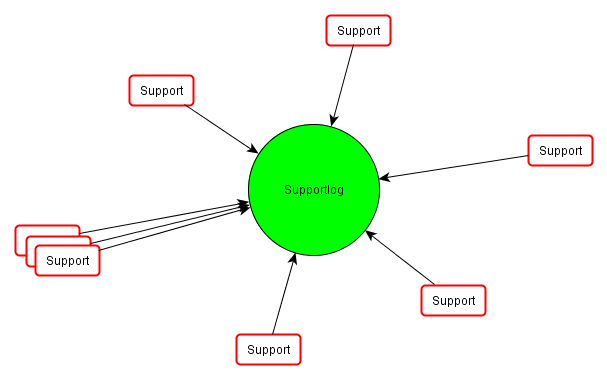
\includegraphics[width=\textwidth]{kapitel/gruppe3/bilder/grafik_supportlog}
	\caption{Unabhängige Supportleister dokumentieren in zentralem Log}
	\label{fig_zentraler_supportlog}
\end{figure}

Die Abbildung \ref{fig_zentraler_supportlog} verdeutlicht, dass geleisteter Support von vollkommen unabhängigen Stellen zentral dokumentiert werden kann.

Es ist dabei unerheblich, ob die Supportleister die Unterstützung als Kern ihrer Aufgabe 
leisten, oder ob es sich um kollegiale Unterstützung bei einem Problem handelt. Gerade 
letztere Information aufzufangen ist wichtig, da diese sonst nur eine sehr schwer 
einzuschätzende Größe bleibt.

Dieser Dokumentationsoverhead ist gering gegenüber dem Overhead eines stark 
reglementierten Supportsystems, erhält alle Vorteile unbürokratischer, schneller 
Hilfeleistung und fängt zusätzlich Informationen über Art und Umfang gelisteten Supports 
auf.

\subsubsection{Knowledge Base}
Aus dem Supportlog kann eine durchsuchbare Knowledge Base aufgebaut werden, die nicht 
nur die allgemeinen Fehlerquellen und Schwierigkeiten von Software im Einsatz beleuchtet, 
sondern ganz speziell die an der Hochschule Emden/Leer in dieser Zusammenstellung 
einmaligen Konfiguration vorliegenden Probleme.

Dadurch kann sehr viel schneller auf spezifische Fehlerszenarien reagiert werden, als dies 
mit allgemeinen Informationen möglich ist, die erst auf die Verhältnisse vor Ort bezogen 
werden müssen.

Auch können aus dem Supportlog FAQs abgeleitet werden, die tatsächlich dem Wortsinn 
nach Listen häufig gestellter Fragen und Antworten darstellen, und nicht was mehr oder 
minder begründet vermutet wird. Eine Diskrepanz mag sich hier durch die Besonderheit von 
Hochschulen ergeben, ein sehr heterogenes Benutzerfeld abzudecken. So mag es 
Nutzergruppen geben, die ein ähnliches Maß an technischer Kompetenz aufweisen wie 
Personal, das ein bestimmtes System betreut, bis hion zu Benutzergruppen, die weit weniger 
oder deutlich andere technische Kompetenz aufweisen.

Auch zeigt sich in den Häufigkeiten bestimmter Probleme, wo spezielle Dokumentation und 
Hilfetexte notwendig sind, die ebenfalls hinterlegt werden können.

Hierzu muss das Supportlog allerdings von einer geeigneten Stelle regelmäßig gesichtet 
werden.

\subsection{Fortentwicklung}
Eine Konzeption kann nur aktuelle Trends und Entwicklungen berücksichtigen. Es ist 
schwierig vorauszuschauen, was die Zukunft danach bringen wird, welche Trends mehr oder 
weniger wichtig sind, und welche Trends darauf folgen werden.

Allerdings ist es keine Frage, dass eine Hochschule länger Bestand hat, und es damit 
sinnvoll ist, Prozesse zu hinterlegen, die neue Trends und Entwicklungen zwar nicht 
vorwegnehmen können, aber deren zeitnahe Entdeckung und Integration ermöglichen.

Auch zeigt sich in der Praxis, dass unvorhergesehene Bedingungen und Ereignisse 
theoretisch gut ausgearbeitete Prozesse und Infrastrukturen übermäßig blockieren können, 
und eine Anpassung geschehen muss. Beispielhaft sei hier für die Hochschule Emden/Leer 
der Trend angeführt, dass Mitarbeiter und Studierende eigene, WLAN-fähige Geräte 
mitbringen und im Netzwerk der Hochschule anzumelden. Das vormals ausreichend 
dimensionierte Netz wurde durch einen Trend unter- oder zumindest 
fehldimensioniert.\footcite{gunter_muller_interview}

\subsubsection{Feedback}
Zur effektiven Begegnung neuer Trends muss an jedem Punkt des Gesamtsystems dem 
Benutzer möglich sein, Feedback zu geben. Mehr noch muss gerade bei neuen oder 
überarbeiteten Prozessen dieses Feedback eingefordert werden, um die Qualität des neuen 
Prozesses oder Tools einschätzen zu können.

Das Feedback gelangt an die zuständige Stelle, muss aber auch zentral gesammelt werden, 
ähnlich wie das Supportlog. Diese Sammlung wird zentral ausgewertet, um verdeckte, 
verteilte Probleme aufzudecken, die sich in Feedback an unterschiedliche Stellen verbergen 
können.

Auf die Auswertung muss, wo sich Probleme zeigen, eine Information der zuständigen Stelle 
folgen, damit eine Verbesserung erarbeitet werden kann. Entsprechend ist die zuständige 
Stelle berechtigt, ein Meeting einzuberufen, damit ihre Eingaben nicht einfach verloren gehen 
können, sondern zwangsläufig mindestens einmal besprochen werden.

\subsubsection{Innovationseingabe}
In den Feedbackprozess eingebettet muss die Möglichkeit für jede Person sein, Innovationen 
aus beliebiger Quelle zu beschreiben, so dass Entwicklungen nicht erst von bestimmter 
Stelle wahrgenommen werden müssen, um erwägt zu werden. Damit kann von beliebiger 
Stelle aus eine Verbesserung in Diskussion gebracht werden.

Damit diese Möglichkeit von Benutzern angenommen wird, muss auf Eingaben angemessen 
schnell reagiert werden. Um eine ernsthafte Reaktion zu gewährleisten, müssen diese 
Vorschläge auch diskutiert worden sein. Daraus ergibt sich ein angemessen kurzer Turnus 
der Auswertung von Support- und Feedbacklog.

\subsubsection{Erfahrungsgetriebene Fortentwicklung}
Aus den Erkenntnissen über Schwachstellen aus dem Supportlog, den Benutzerberichten und 
-bewertungen aus dem Feedbacklog und den Innovationseingaben können nicht nur 
Schwachstellen und Fehler in Prozessen identifiziert werden, sondern auch Trends in der 
Benutzung des Systems erkannt. Da Support und Feedback andauernde Prozesse sind, ergibt 
sich daraus ein selbstregulierendes System, das, wenn die Messgrößen Supportlog und 
Feedbacklog angemessen berücksichtigt werden, evolutionär verbessert wird.

\begin{figure}[h!]
	\centering
	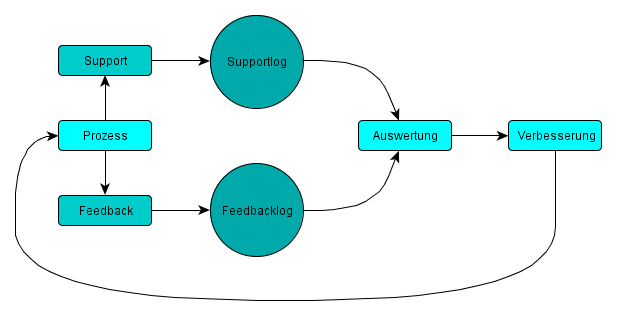
\includegraphics[width=\textwidth]{kapitel/gruppe3/bilder/zyklus_prozessverbesserung}
	\caption{Zyklus der Verbesserung eines Prozesses}
	\label{fig_zyklus_prozessverbesserung}
\end{figure}

Abbildung \ref{fig_zyklus_prozessverbesserung} illustriert den Zyklus folgendermaßen: Ein Prozess existiert und läuft im 
normalen Betrieb. Bei Problemen wird Support geleistet, der im Supportlog vermerkt wird. Zu 
dem Prozess wird zusätzlich Feedback gegeben, das im Feedbacklog festgehalten wird. Beide 
Logs werden ausgewertet und zur Verbesserung des Prozesses herangezogen. Der 
verbesserte Prozess tritt an die Stelle des ursprünglichen Prozesses, der Zyklus beginnt auf 
Basis des verbesserten Prozesses erneut.




















